\documentclass[../main.tex]{subfiles}
\begin{document}
\chapter{Resultados}
Para conseguir resultados significativos, no sólo debieron seguirse los métodos descritos en el capítulo anterior, sino que también estos se realizaron en un orden particular, que permitió determinar las condiciones de las técnicas subsecuentes además de prevenir mediciones innecesarias. En la figura \ref{fig:resdiag} se puede observar un diagrama del orden seguido.
\begin{figure}[H]
    \centering
    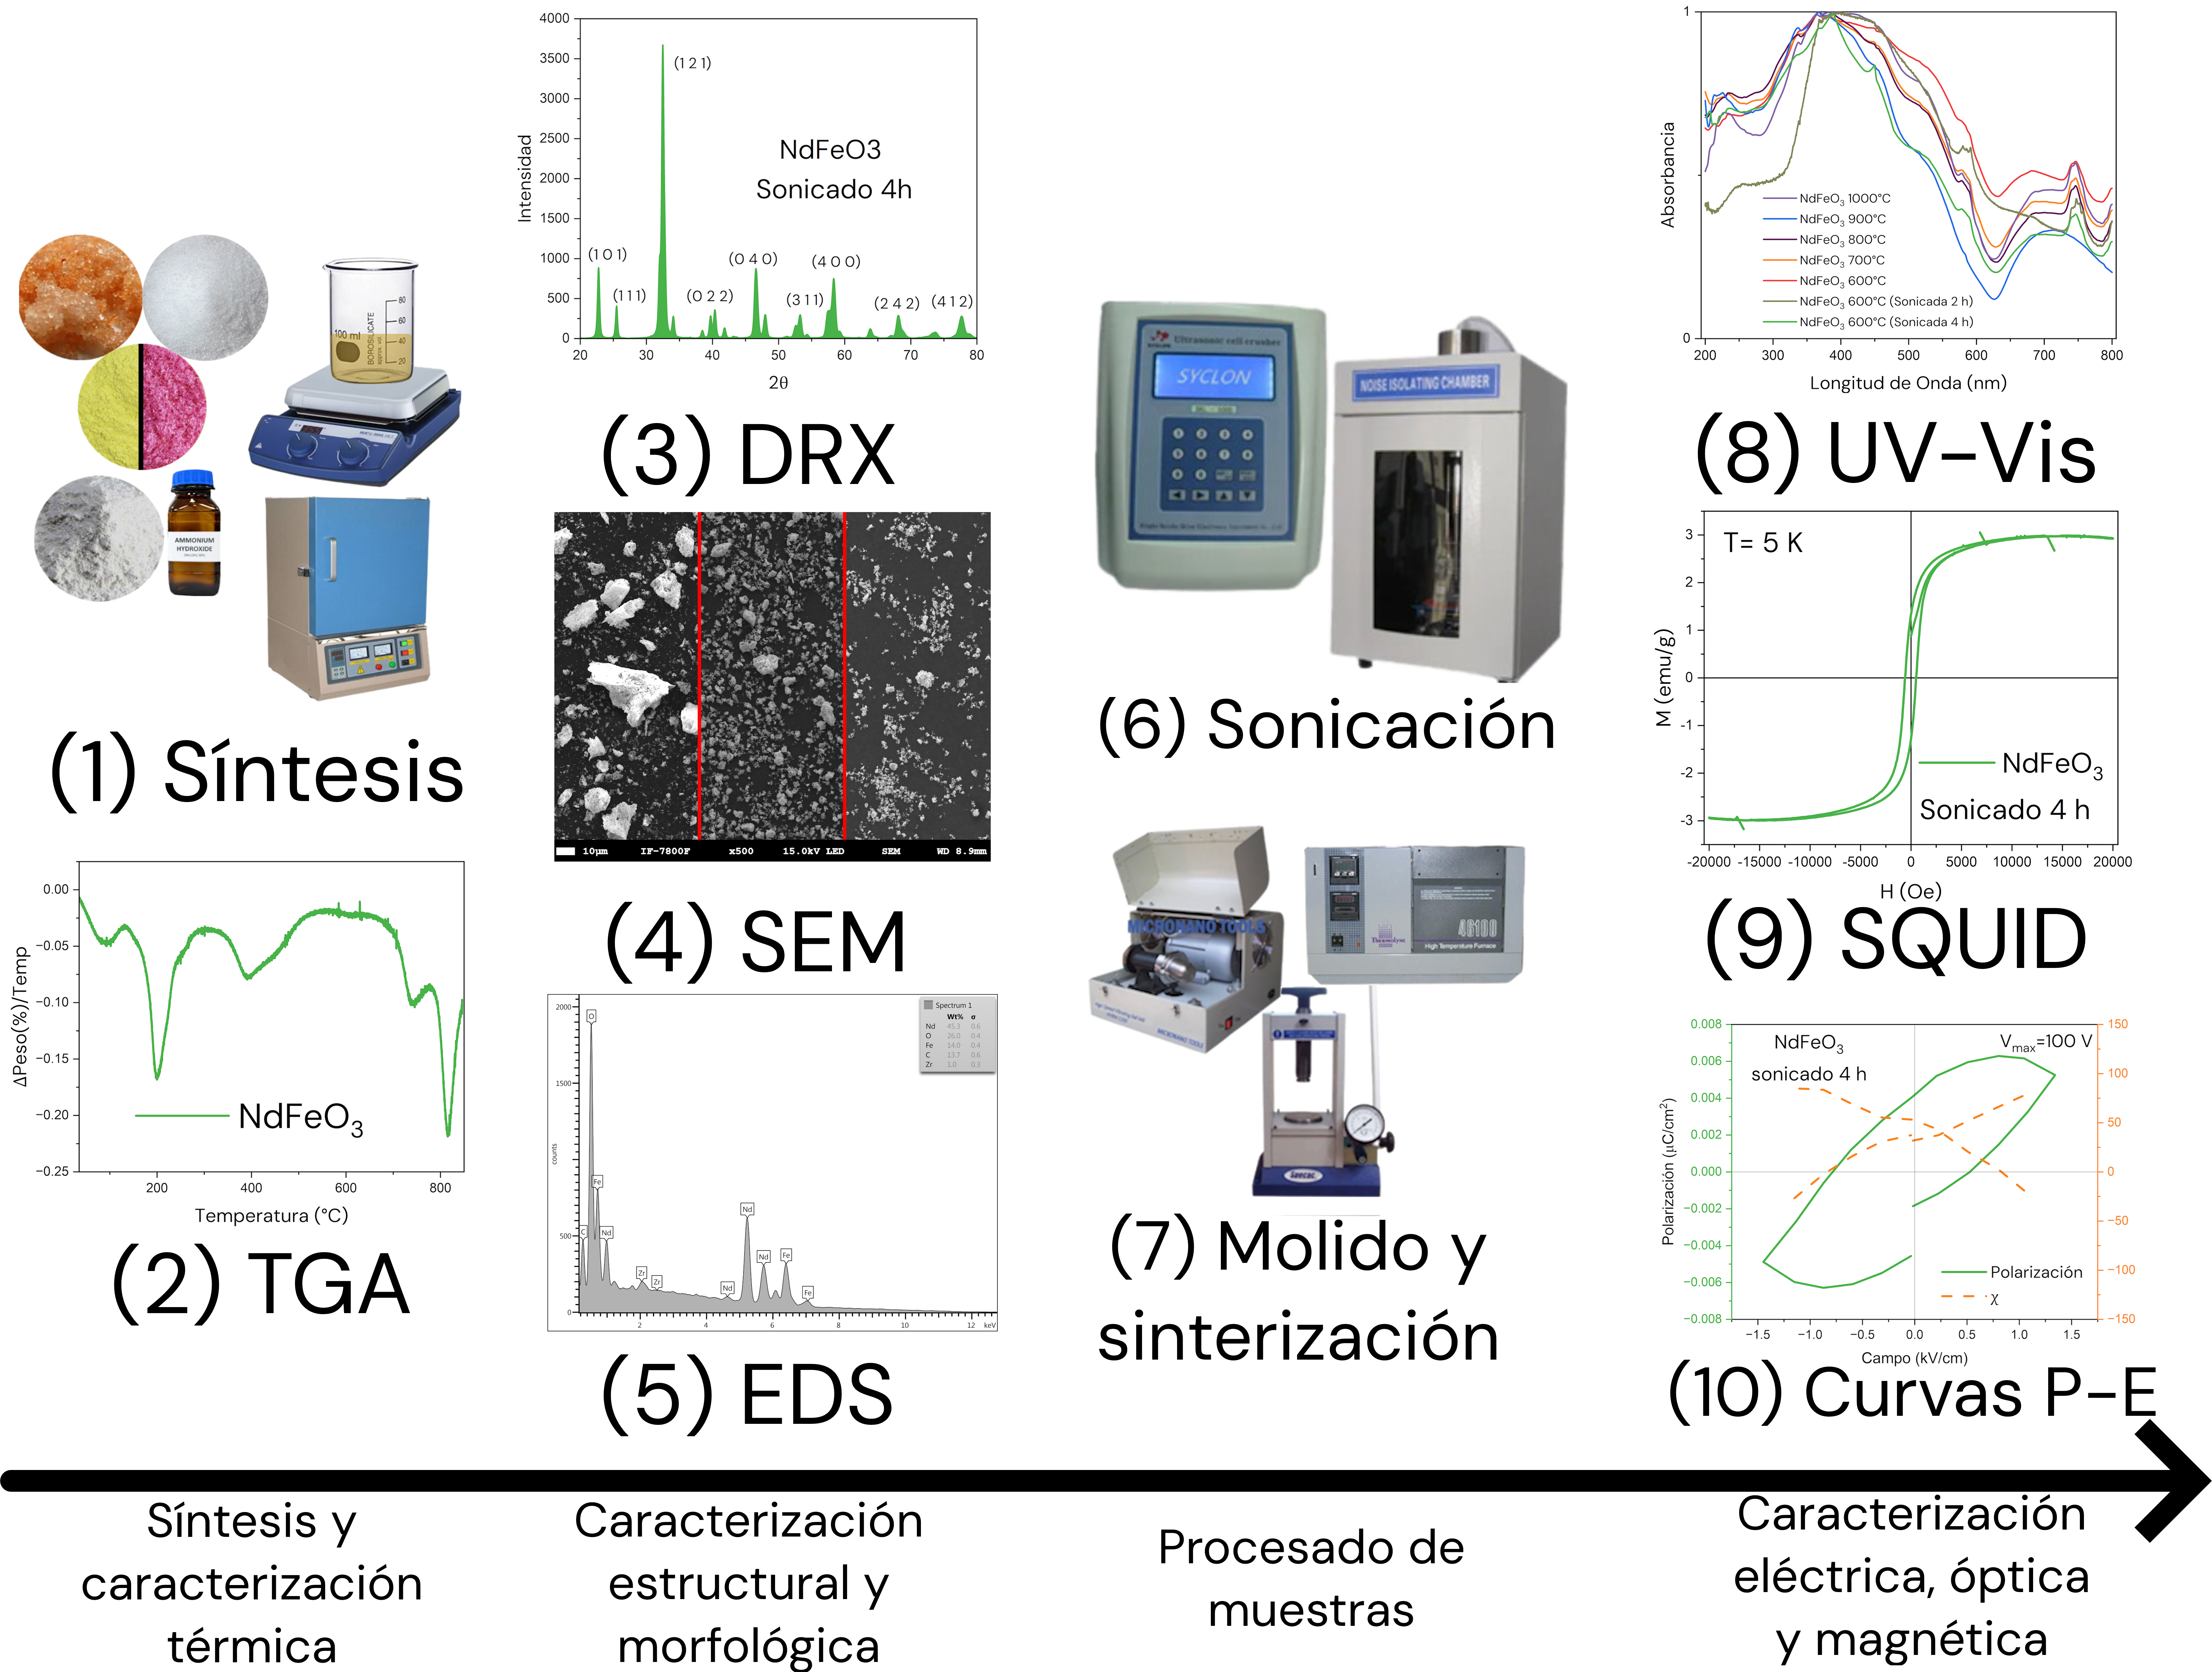
\includegraphics[width=0.7\textwidth]{fig/diagresultados.png}
    \caption{Resultados obtenidos mediante las técnicas de síntesis y caracterización descritas en el capítulo 4.}
    \label{fig:resdiag}
\end{figure}
\section{Muestras Sintetizadas} \label{sec:sintesis}
Se sintetizaron un total de 9 muestras de 1gr de \neod{} y 8 de \sama{}. Una muestra de cada ortoferrita fue reservada para realizar un análisis termogravimétrico. A través de éste, se determinó la temperatura mínima de calcinación para ambas ortoferritas, como se reporta en la sección \ref{sec:TGA}.

Con estas temperaturas en mente, 600\gradoC{} para el \neod{} y 700\gradoC{} para el \sama{}, se calcinaron el resto de muestras, 4 muestras de \neod{} se calcinaron a 600\gradoC{}, para las otras 4 se aumentó la temperatura 100\gradoC{} por cada una, es decir, se calcinaron a 700, 800, 900 y 1000\gradoC{} respectivamente.

Por otro lado, para el \sama{} se calcinaron 4 muestras a 700\gradoC{}, aumentando la temperatura de la misma forma que en el caso del \neod{} para las otras 3, es decir, se calcinaron a 800, 900 y 1000\gradoC{} respectivamente.
\section{Caracterización}
Las técnicas realizadas en esta sección pueden dividirse en tres apartados. Análisis térmico (sección \ref{sec:analisistermico}), que permite optimizar las condiciones de síntesis, análisis estructural, morfológico y de composición (sección \ref{sec:analisisestruc}), que permite comprobar la presencia de la fase que se busca y estudiar la forma física de las muestras sintetizadas y, finalmente, análisis óptico, magnético y eléctrico (sección \ref{sec:analisisoptmagelec}), con el fin de relacionar estas propiedades con las estudiadas en la sección anterior. En conjunto, estos análisis permiten una caracterización apropiada de las muestras obtenidas en función del tamaño de partícula.
\subsection{Análisis Térmico} \label{sec:analisistermico}
\subsubsection{Análisis Termogravimétrico} \label{sec:TGA}

\subsection{Análisis Estructural, Morfológico y de Composición} \label{sec:analisisestruc}

\subsubsection{Microscopía Electrónica de Barrido}
Se estudió la morfología de las partículas sintetizadas a través de esta técnica, dando como resultado imágenes como las que se muestran en la figura %\ref{fig:resSEM}.

Inicialmente se comparó sólo el tamaño de partícula según el tamaño de calcinación, lo cual, como se muestra en la figura \ref{fig:resTamaños}, no dió como resultado una relación clara. A raíz de ésto, se prepararon muestras sonicadas a partir de las calcinadas a más baja temperatura para cada tierra rara.

En general, se observa que estas partículas presentan una estructura porosa, la cual se rompe después de ser sometida a un proceso de sonicación, siendo esto evidente al comparar las figuras \ref{fig:resSEMsonic} (a) y\ref{fig:resSEMsonic} (b), las cuales muestras a las ortoferritas de \neod{} calcinada a 600\gradoC{} y \sama{} calcinada a 700\gradoC{} respectivamente, con las figuras \ref{fig:resSEMsonic} (c) y\ref{fig:resSEMsonic}(d), en donde se muestran éstas mismas muestras después de ser sonicadas por 2 horas a 292W, además de las figuras \ref{fig:resSEMsonic} (e) y \ref{fig:resSEMsonic} (f), donde éstas muestras fueron sonicadas por 4 horas a la misma potencia.
\begin{figure}[H]
    \centering
    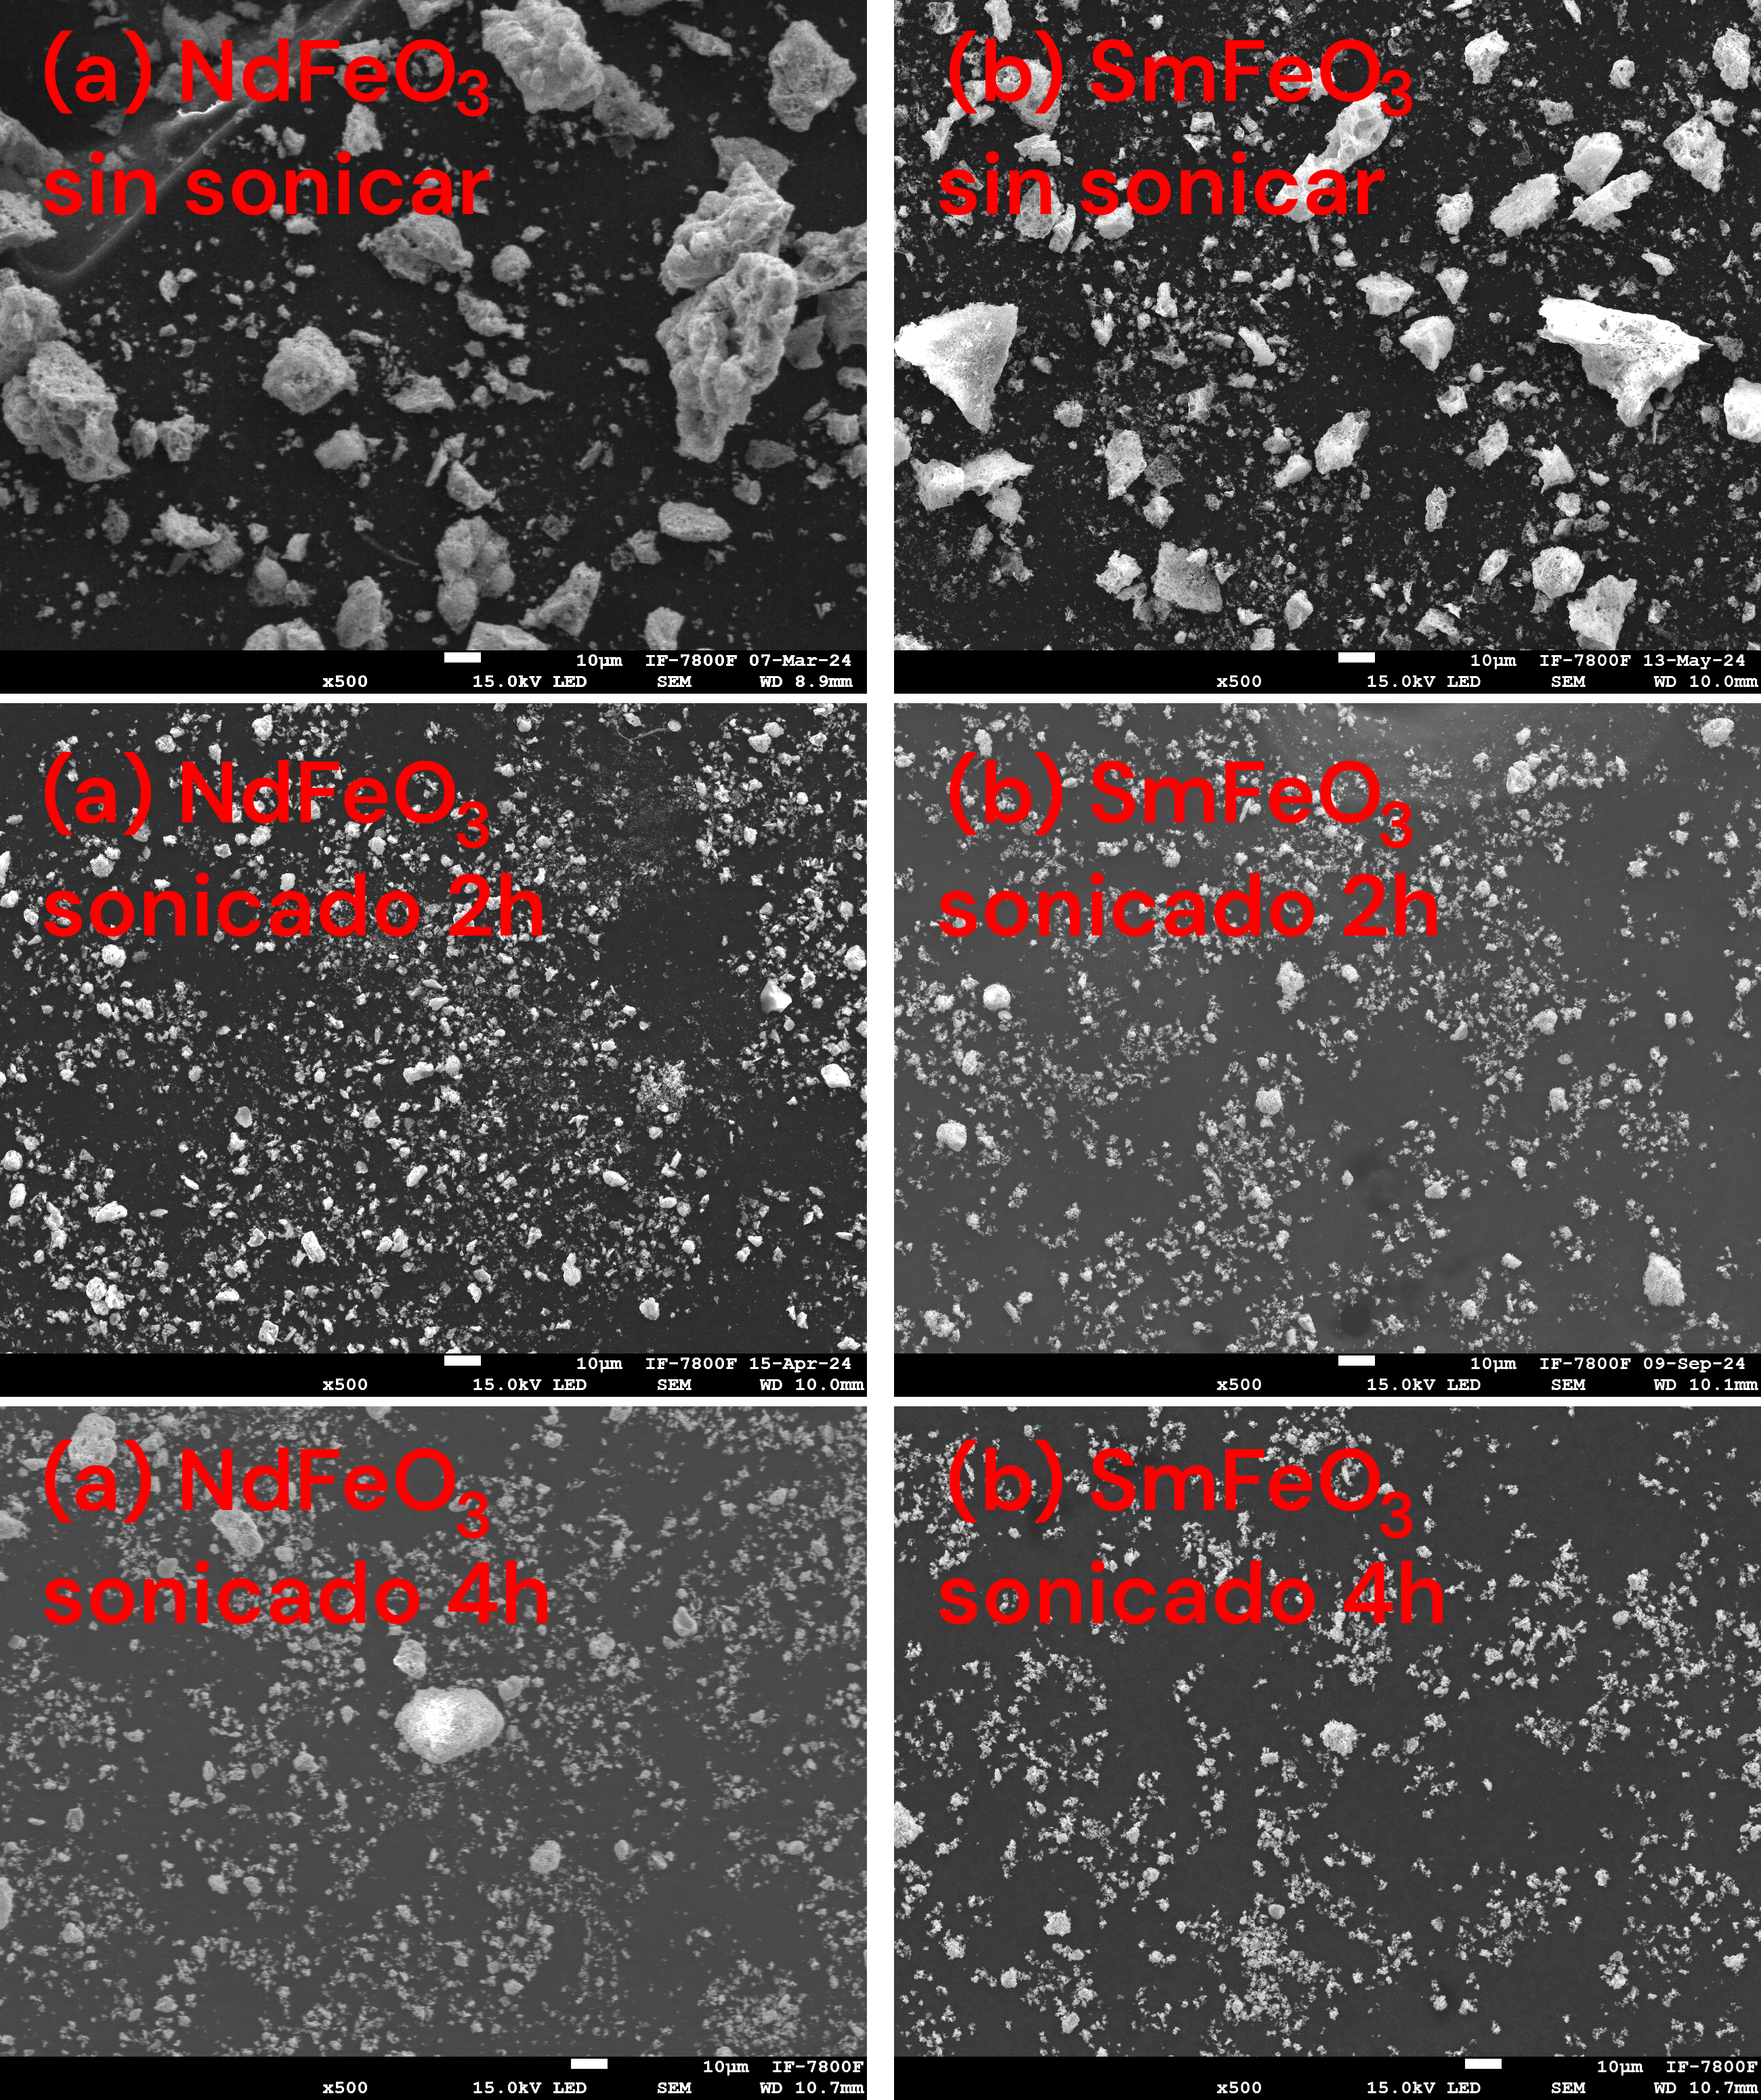
\includegraphics[width=0.7\textwidth]{fig/ressem.png}
    \caption{Imágenes obtenidas a través de SEM. Amplificación x500.}
    \label{fig:resSEMsonic}
\end{figure}
Como ya se describió en el capítulo \ref{sec:analisisestadistico}, los tamaños de partícula fueron obtenidos haciendo uso de \textit{ImageJ}, dando como resultado los histogramas presentados en la figura %\ref{fig:reshist}
%\begin{figure}[H]
%    \centering
%    \includegraphics[width=0.8\textwidth]{fig/reshist.png}
%    \caption{Histogramas obtenidos.}
%    \label{fig:reshist}
%\end{figure}
Finalmente, a través de los datos obtenidos, se siguió el método ya descrito en la sección \ref{sec:analisisestadistico}, lo cual dió como resultado los siguientes datos.
\begin{figure}[H]
    \centering
    \includegraphics[width=0.9\textwidth]{fig/resTamaños.png}
    \caption{Tamaño de partícula según su temperatura de calcinación.}
    \label{fig:resTamaños}
\end{figure}
\subsubsection{Espectroscopía de Dispersión de Energía}
Esta técnica reveló los elementos presentes en las muestras introducidas al microscopio electrónico de barrido, lo cual permite hallar posibles contaminantes, además de delimitar las posibles estructuras cristalinas a tomar en cuenta en el análisis de la difracción de rayos X de la sección \ref{sec:analisisDRX}.

En ninguna de las mediciones se encontraron contaminantes externos, a excepción de carbono, el cuál puede explicarse debido a que la cinta utilizada para la preparación de muestras está hecha de este material, esto se reporta en las tablas \ref{tab:EDSNd} y \ref{tab:EDSSm}.

\begin{table}[H]
    \begin{tabular}{|c||c|c|c|c|c|c|c|}
        \hline
        Elem. &600\gradoC{} Son.&600\gradoC{} Son.&600\gradoC{}&700\gradoC{}&800\gradoC{}&900\gradoC{}&1000\gradoC{}\\
        &2h wt\%&4h wt\%&wt\%&wt\%&wt\%&wt\%&wt\%\\
        \hline\hline
        Fe & 20.33$\pm$0.78 &$21.00\pm0.77$& 19.94$\pm$0.68 & 22.23$\pm$1.01 & 20.31$\pm$0.67 & 21.0$\pm$1.04 & 18.37$\pm$2.06 \\
        Nd & 47.88$\pm$0.92 &$58.44\pm0.87$& 50.45$\pm$0.85 & 58.93$\pm$1.21 & 56.47$\pm$0.83 & 44.7$\pm$1.18 & 78.72$\pm$2.12 \\
        O & 31.79$\pm$0.70 &$20.56\pm0.56$& 21.71$\pm$0.54 & 11.04$\pm$0.57 & 15.06$\pm$0.45 & 20.4$\pm$0.57 & 2.92$\pm$0.60 \\
        C & 0 & 0 & 7.91$\pm$0.64 & 7.8$\pm$0.82 & 8.16$\pm$0.56 & 13.4$\pm$0.67 &0 \\ 
        \hline
        \end{tabular} 
            \caption{EDS de las muestras de \neod{}.}
            \label{tab:EDSNd}
        \end{table}
        \begin{table}[H]
            \centering
        \begin{tabular}{|c||c|c|c|c|c|c|}
        \hline
        Elem. &700\gradoC{} Son.&700\gradoC{} Son.&700\gradoC{}&800\gradoC{}&900\gradoC{}&1000\gradoC{}\\
        &2h wt\%&4h wt\%&wt\%&wt\%&wt\%&wt\%\\
        \hline\hline
        Fe &$13.78\pm0.52$&$19.48\pm1.48$& 7.51$\pm$0.42 & 22.31$\pm$0.93 & 22.51$\pm$3.03 & 17.44$\pm$0.83 \\
        Sm &$38.42\pm0.74$&$48.22\pm1.95$& 21.84$\pm$0.69 & 61.28$\pm$1.03 & 63.03$\pm$3.57 & 57.71$\pm$1.82 \\
        O &$18.74\pm0.45$&$15.64\pm1.00$& 15.95$\pm$0.47 & 16.41$\pm$0.58 & 14.46$\pm$1.78 & 20.81$\pm$0.78 \\
        C &$29.16\pm0.62$&$16.66\pm1.53$& 0 & 54.68$\pm$0.77 & 0 & 4.13$\pm$2.17 \\ 
        \hline
        \end{tabular} 
            \caption{EDS de las muestras de \sama{}.}
            \label{tab:EDSSm}
\end{table}

\subsubsection{Difracción de Rayos X} \label{sec:analisisDRX}


\subsection{Análisis Óptico, Magnético y Eléctrico} \label{sec:analisisoptmagelec}
\subsubsection{Espectroscopía UV-Vis}

\subsubsection{Magnetometría VSM}

\paragraph{M vs T}

\paragraph{\textchi{} vs T}

\paragraph{M v H}
\subsubsection{Espectroscopía de Impedancia}
\end{document}